\newpage
\subsection{Caso d'uso UC11: Registrazione nuova API}
\label{UC11}
\begin{figure}[ht]
	\centering
	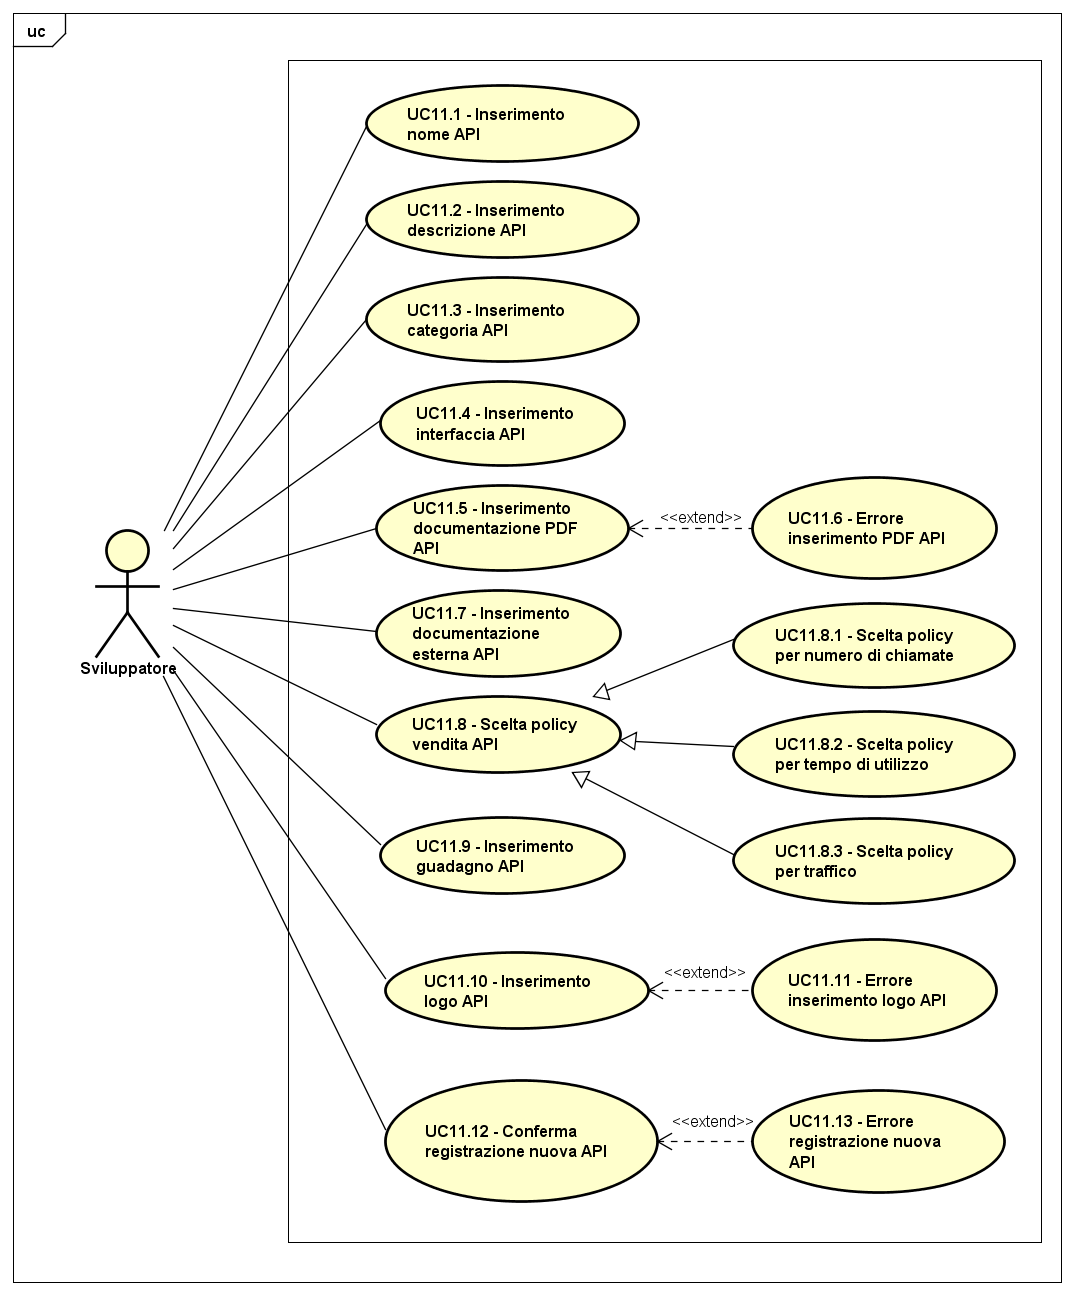
\includegraphics[scale=0.45]{UML/UC11.png}
	\caption{UC11: Registrazione nuova API}
\end{figure}

\begin{longtable}{ l | p{11cm}}
	\hline
	\rowcolor{Gray}
	\multicolumn{2}{c}{UC11 - Registrazione nuova API}\\
	\hline
	\textbf{Attori} & Sviluppatore \\
	\textbf{Descrizione} & L'attore registra una nuova API su API Market \\
	\textbf{Pre-Condizioni} & L'attore si trova nella schermata relativa alla registrazione di una nuova API \\
	\textbf{Post-Condizioni} & L'attore ha registrato una nuova API su API Market \\
	\textbf{Scenario Principale} & 
	\begin{enumerate*}[label=(\arabic*.),itemjoin={\newline}]
		\item L'attore può inserire il nome della nuova API (UC11.1)
		\item L'attore può inserire la descrizione della nuova API (UC11.2)
		\item L'attore può inserire la categoria della nuova API (UC11.3)
		\item L'attore può inserire l'interfaccia della nuova API (UC11.4)
		\item L'attore può inserire il file per la documentazione PDF della nuova API (UC11.5)
		\item L'attore può inserire il link per la documentazione esterna della nuova API (UC11.7)
		\item L'attore può scegliere la policy di vendita della nuova API (UC11.8)
		\item L'attore può inserire il guadagno netto desiderato per la nuova API (UC11.9)
		\item L'attore può inserire il file per il logo della nuova API (UC11.10)
		\item L'attore può confermare la registrazione della nuova API (UC11.12)
	\end{enumerate*}\\
	\textbf{Scenari Alternativi} & 
	\begin{enumerate*}[label=(\arabic*.),itemjoin={\newline}]
			\item L'attore può visualizzare un messaggio di errore riguardo al caricamento del file di documentazione PDF della nuova API, ed il caricamento del file non avviene (UC11.6)
			\item L'attore può scegliere la licenza API per numero di chiamate (UC11.8.1)
			\item L'attore può scegliere la licenza API per tempo di utilizzo (UC11.8.2)
			\item L'attore può scegliere la licenza API per traffico (UC11.8.3)
			\item L'attore può visualizzare un messaggio di errore riguardo al caricamento del file del logo della nuova API, ed il caricamento del file non avviene (UC11.11)
			\item L'attore, dopo aver confermato la registrazione della nuova API, può visualizzare un messaggio d'errore informativo e la registrazione non avviene (UC11.13)
	\end{enumerate*}\\
\end{longtable}

\subsubsection{Caso d'uso UC11.1: Inserimento nome API}
\label{UC11_1}

\begin{minipage}{\linewidth}
	\begin{tabular}{ l | p{11cm}}
		\hline
		\rowcolor{Gray}
		\multicolumn{2}{c}{UC11.1 - Inserimento nome API} \\
		\hline
		\textbf{Attori} & Sviluppatore \\
		\textbf{Descrizione} & L'attore inserisce il nome della nuova API \\
		\textbf{Pre-Condizioni} & L'attore si trova nella schermata relativa alla registrazione di una nuova API \\
		\textbf{Post-Condizioni} & L'attore ha inserito il nome della nuova API \\
		\textbf{Scenario Principale} & 
		\begin{enumerate*}[label=(\arabic*.),itemjoin={\newline}]
			\item L'attore può inserire il nome della nuova API
		\end{enumerate*}\\
	\end{tabular}
\end{minipage}

\subsubsection{Caso d'uso UC11.2: Inserimento descrizione API}
\label{UC11_2}

\begin{minipage}{\linewidth}
	\begin{tabular}{ l | p{11cm}}
		\hline
		\rowcolor{Gray}
		\multicolumn{2}{c}{UC11.2 - Inserimento descrizione API} \\
		\hline
		\textbf{Attori} & Sviluppatore \\
		\textbf{Descrizione} & L'attore inserisce la descrizione della nuova API \\
		\textbf{Pre-Condizioni} & L'attore si trova nella schermata relativa alla registrazione di una nuova API \\
		\textbf{Post-Condizioni} & L'attore ha inserito la descrizione della nuova API \\
		\textbf{Scenario Principale} & 
		\begin{enumerate*}[label=(\arabic*.),itemjoin={\newline}]
			\item L'attore può inserire la descrizione della nuova API
		\end{enumerate*}\\
	\end{tabular}
\end{minipage}

\subsubsection{Caso d'uso UC11.3: Inserimento categoria API}
\label{UC11_3}

\begin{minipage}{\linewidth}
	\begin{tabular}{ l | p{11cm}}
		\hline
		\rowcolor{Gray}
		\multicolumn{2}{c}{UC11.3 - Inserimento categoria API} \\
		\hline
		\textbf{Attori} & Sviluppatore \\
		\textbf{Descrizione} & L'attore inserisce la categoria della nuova API \\
		\textbf{Pre-Condizioni} & L'attore si trova nella schermata relativa alla registrazione di una nuova API \\
		\textbf{Post-Condizioni} & L'attore ha inserito la categoria della nuova API \\
		\textbf{Scenario Principale} & 
		\begin{enumerate*}[label=(\arabic*.),itemjoin={\newline}]
			\item L'attore può inserire la categoria della nuova API
		\end{enumerate*}\\
	\end{tabular}
\end{minipage}

\subsubsection{Caso d'uso UC11.4: Inserimento interfaccia API}
\label{UC11_4}

\begin{minipage}{\linewidth}
	\begin{tabular}{ l | p{11cm}}
		\hline
		\rowcolor{Gray}
		\multicolumn{2}{c}{UC11.4 - Inserimento interfaccia API} \\
		\hline
		\textbf{Attori} & Sviluppatore \\
		\textbf{Descrizione} & L'attore inserisce l'interfaccia della nuova API \\
		\textbf{Pre-Condizioni} & L'attore si trova nella schermata relativa alla registrazione di una nuova API \\
		\textbf{Post-Condizioni} & L'attore ha inserito l'interfaccia della nuova API \\
		\textbf{Scenario Principale} & 
		\begin{enumerate*}[label=(\arabic*.),itemjoin={\newline}]
			\item L'attore può inserire l'interfaccia della nuova API
		\end{enumerate*}\\
	\end{tabular}
\end{minipage}

\subsubsection{Caso d'uso UC11.5: Inserimento documentazione PDF API}
\label{UC11_5}

\begin{minipage}{\linewidth}
	\begin{tabular}{ l | p{11cm}}
		\hline
		\rowcolor{Gray}
		\multicolumn{2}{c}{UC11.5 - Inserimento documentazione PDF API} \\
		\hline
		\textbf{Attori} & Sviluppatore \\
		\textbf{Descrizione} & L'attore carica su API Market un file PDF contenente la documentazione PDF della nuova API \\
		\textbf{Pre-Condizioni} & L'attore si trova nella schermata relativa alla registrazione di una nuova API \\
		\textbf{Post-Condizioni} & L'attore ha caricato su API Market un file PDF contenente la documentazione PDF della nuova API \\
		\textbf{Scenario Principale} & 
		\begin{enumerate*}[label=(\arabic*.),itemjoin={\newline}]
			\item L'attore può caricare su API Market un file PDF contenente la documentazione PDF della nuova API
		\end{enumerate*}\\
		\textbf{Scenari Alternativi} & 
		\begin{enumerate*}[label=(\arabic*.),itemjoin={\newline}]
		\item L'attore può visualizzare un messaggio di errore (E.g: formato errato) ed il caricamento del file non avviene (UC11.10)
		\end{enumerate*}\\
	\end{tabular}
\end{minipage}

\subsubsection{Caso d'uso UC11.6: Errore inserimento PDF API}
\label{UC11_6}

\begin{minipage}{\linewidth}
	\begin{tabular}{ l | p{11cm}}
		\hline
		\rowcolor{Gray}
		\multicolumn{2}{c}{UC11.6 - Errore inserimento PDF API} \\
		\hline
		\textbf{Attori} & Sviluppatore \\
		\textbf{Descrizione} & L'attore visualizza un messaggio di errore e l'inserimento della documentazione PDF della nuova API non avviene \\
		\textbf{Pre-Condizioni} & L'attore ha cercato di caricare su API Market un file contenente la documentazione della nuova API ma si è verificato un errore \\
		\textbf{Post-Condizioni} & L'attore ha visualizzato un messaggio di errore \\
		\textbf{Scenario Principale} & 
		\begin{enumerate*}[label=(\arabic*.),itemjoin={\newline}]
			\item L'attore può visualizzare un messaggio di errore
		\end{enumerate*}\\
	\end{tabular}
\end{minipage}

\subsubsection{Caso d'uso UC11.7: Inserimento documentazione esterna API}
\label{UC11_7}

\begin{minipage}{\linewidth}
	\begin{tabular}{ l | p{11cm}}
		\hline
		\rowcolor{Gray}
		\multicolumn{2}{c}{UC11.7 - Inserimento documentazione esterna API} \\
		\hline
		\textbf{Attori} & Sviluppatore \\
		\textbf{Descrizione} & L'attore inserisce il link alla documentazione esterna della nuova API \\
		\textbf{Pre-Condizioni} & L'attore si trova nella schermata relativa alla registrazione di una nuova API \\
		\textbf{Post-Condizioni} & L'attore ha inserito il link alla documentazione esterna della nuova API \\
		\textbf{Scenario Principale} & 
		\begin{enumerate*}[label=(\arabic*.),itemjoin={\newline}]
			\item L'attore può inserire il link alla documentazione esterna della nuova API
		\end{enumerate*}\\
	\end{tabular}
\end{minipage}

\subsubsection{Caso d'uso UC11.8: Scelta policy vendita API}
\label{UC9_2}

\begin{minipage}{\linewidth}
	\begin{tabular}{ l | p{11cm}}
		\hline
		\rowcolor{Gray}
		\multicolumn{2}{c}{UC11.8.2 - Scelta policy vendita API} \\
		\hline
		\textbf{Attori} & Sviluppatore \\
		\textbf{Descrizione} & L'attore sceglie una policy di vendita per la nuova API \\
		\textbf{Pre-Condizioni} & L'attore si trova nella schermata di registrazione di una nuova API \\
		\textbf{Post-Condizioni} & L'attore ha scelto una policy di vendita per la nuova API \\
		\textbf{Scenario Principale} & 
		\begin{enumerate*}[label=(\arabic*.),itemjoin={\newline}]
			\item L'attore può scegliere una policy di vendita per la nuova API
		\end{enumerate*}\\
		\textbf{Scenari Alternativi} & 
		\begin{enumerate*}[label=(\arabic*.),itemjoin={\newline}]
			\item L'attore può scegliere la policy di vendita per numero di chiamate (UC11.8.1)
			\item L'attore può scegliere la policy di vendita per tempo di utilizzo (UC11.8.2)
			\item L'attore può scegliere la policy di vendita per traffico (UC11.8.3)	
		\end{enumerate*}\\
	\end{tabular}
\end{minipage}

\paragraph{Caso d'uso UC11.8.1: Scelta policy per numero di chiamate}
\label{UC11_8_1}

\begin{minipage}{\linewidth}
	\begin{tabular}{ l | p{11cm}}
		\hline
		\rowcolor{Gray}
		\multicolumn{2}{c}{UC11.8.1 - Scelta policy per numero di chiamate} \\
		\hline
		\textbf{Attori} & Sviluppatore \\
		\textbf{Descrizione} & L'attore sceglie la policy di vendita API per numero di chiamate \\
		\textbf{Pre-Condizioni} & L'attore si trova nella schermata di registrazione di una nuova API \\
		\textbf{Post-Condizioni} & L'attore ha scelto la policy di vendita API per numero di chiamate \\
		\textbf{Scenario Principale} & 
		\begin{enumerate*}[label=(\arabic*.),itemjoin={\newline}]
			\item L'attore può scegliere la policy di vendita API per numero di chiamate
		\end{enumerate*}\\
	\end{tabular}
\end{minipage}

\paragraph{Caso d'uso UC11.8.2: Scelta policy per tempo di utilizzo}
\label{UC11_8_2}

\begin{minipage}{\linewidth}
	\begin{tabular}{ l | p{11cm}}
		\hline
		\rowcolor{Gray}
		\multicolumn{2}{c}{UC11.8.2 - Scelta policy per tempo di utilizzo} \\
		\hline
		\textbf{Attori} & Sviluppatore \\
		\textbf{Descrizione} & L'attore sceglie la policy di vendita API per tempo di utilizzo \\
		\textbf{Pre-Condizioni} & L'attore si trova nella schermata di registrazione di una nuova API \\
		\textbf{Post-Condizioni} & L'attore ha scelto la policy di vendita API per tempo di utilizzo \\
		\textbf{Scenario Principale} & 
		\begin{enumerate*}[label=(\arabic*.),itemjoin={\newline}]
			\item L'attore può scegliere la policy di vendita API per tempo di utilizzo
		\end{enumerate*}\\
	\end{tabular}
\end{minipage}

\paragraph{Caso d'uso UC11.8.3: Scelta policy per traffico}
\label{UC11_8_3}

\begin{minipage}{\linewidth}
	\begin{tabular}{ l | p{11cm}}
		\hline
		\rowcolor{Gray}
		\multicolumn{2}{c}{UC11.8.3 - Scelta policy per traffico} \\
		\hline
		\textbf{Attori} & Sviluppatore \\
		\textbf{Descrizione} & L'attore sceglie la policy di vendita API per traffico \\
		\textbf{Pre-Condizioni} & L'attore si trova nella schermata di registrazione di una nuova API \\
		\textbf{Post-Condizioni} & L'attore ha scelto la policy di vendita API per traffico \\
		\textbf{Scenario Principale} & 
		\begin{enumerate*}[label=(\arabic*.),itemjoin={\newline}]
			\item L'attore può scegliere la policy di vendita API per traffico
		\end{enumerate*}\\
	\end{tabular}
\end{minipage}

\subsubsection{Caso d'uso UC11.9: Inserimento guadagno API}
\label{UC11_9}

\begin{minipage}{\linewidth}
	\begin{tabular}{ l | p{11cm}}
		\hline
		\rowcolor{Gray}
		\multicolumn{2}{c}{UC11.9 - Inserimento guadagno API} \\
		\hline
		\textbf{Attori} & Sviluppatore \\
		\textbf{Descrizione} & L'attore inserisce il guadagno netto desiderato per la nuova API \\
		\textbf{Pre-Condizioni} & L'attore si trova nella schermata relativa alla registrazione di una nuova API \\
		\textbf{Post-Condizioni} & L'attore ha inserito il guadagno netto desiderato per la nuova API \\
		\textbf{Scenario Principale} & 
		\begin{enumerate*}[label=(\arabic*.),itemjoin={\newline}]
			\item L'attore può inserire il guadagno netto desiderato per la nuova API
		\end{enumerate*}\\
	\end{tabular}
\end{minipage}

\subsubsection{Caso d'uso UC11.10: Inserimento logo API}
\label{UC11_10}

\begin{minipage}{\linewidth}
	\begin{tabular}{ l | p{11cm}}
		\hline
		\rowcolor{Gray}
		\multicolumn{2}{c}{UC11.10 - Inserimento logo API} \\
		\hline
		\textbf{Attori} & Sviluppatore \\
		\textbf{Descrizione} & L'attore carica su API Market un file contenente il logo per la nuova API \\
		\textbf{Pre-Condizioni} & L'attore si trova nella schermata relativa alla registrazione di una nuova API \\
		\textbf{Post-Condizioni} & L'attore ha caricato su API Market un file contenente il logo per la nuova API \\
		\textbf{Scenario Principale} & 
		\begin{enumerate*}[label=(\arabic*.),itemjoin={\newline}]
			\item L'attore può caricare su API Market un file contenente il logo per la nuova API
		\end{enumerate*}\\
		\textbf{Scenari Alternativi} & 
		\begin{enumerate*}[label=(\arabic*.),itemjoin={\newline}]
		\item L'attore può visualizzare un messaggio di errore (E.g: formato errato) ed il caricamento del file non avviene (UC11.11)
		\end{enumerate*}\\
	\end{tabular}
\end{minipage}

\subsubsection{Caso d'uso UC11.11: Errore inserimento logo API}
\label{UC11_11}

\begin{minipage}{\linewidth}
	\begin{tabular}{ l | p{11cm}}
		\hline
		\rowcolor{Gray}
		\multicolumn{2}{c}{UC11.11 - Errore inserimento logo API} \\
		\hline
		\textbf{Attori} & Sviluppatore \\
		\textbf{Descrizione} & L'attore visualizza un messaggio di errore e l'inserimento del logo per la nuova API non avviene \\
		\textbf{Pre-Condizioni} & L'attore ha cercato di caricare su API Market un file contenente il logo per la nuova API ma si è verificato un errore \\
		\textbf{Post-Condizioni} & L'attore ha visualizzato un messaggio di errore \\
		\textbf{Scenario Principale} & 
		\begin{enumerate*}[label=(\arabic*.),itemjoin={\newline}]
			\item L'attore può visualizzare un messaggio di errore (E.g: formato non valido)
		\end{enumerate*}\\
	\end{tabular}
\end{minipage}

\subsubsection{Caso d'uso UC11.12: Conferma registrazione nuova API}
\label{UC11_12}

\begin{minipage}{\linewidth}
	\begin{tabular}{ l | p{11cm}}
		\hline
		\rowcolor{Gray}
		\multicolumn{2}{c}{UC11.12 - Conferma registrazione nuova API} \\
		\hline
		\textbf{Attori} & Sviluppatore \\
		\textbf{Descrizione} & L'attore conferma la registrazione della nuova API \\
		\textbf{Pre-Condizioni} & L'attore si trova nella schermata relativa alla registrazione di una nuova API \\
		\textbf{Post-Condizioni} & L'attore ha confermato la registrazione della nuova API \\
		\textbf{Scenario Principale} & 
		\begin{enumerate*}[label=(\arabic*.),itemjoin={\newline}]
			\item L'attore può confermare la registrazione della nuova API, visualizzando un messaggio di successo e venendo reindirizzato alla schermata di visualizzazione API registrate (UC10)
		\end{enumerate*}\\
	\end{tabular}
\end{minipage}

\subsubsection{Caso d'uso UC11.13: Errore registrazione nuova API}
\label{UC11_13}

\begin{minipage}{\linewidth}
	\begin{tabular}{ l | p{11cm}}
		\hline
		\rowcolor{Gray}
		\multicolumn{2}{c}{UC11.13 - Errore registrazione nuova API} \\
		\hline
		\textbf{Attori} & Sviluppatore \\
		\textbf{Descrizione} & L'attore visualizza un messaggio di errore informativo e la registrazione della nuova API non avviene \\
		\textbf{Pre-Condizioni} & L'attore ha confermato la registrazione della una nuova API ma si è verificato un errore \\
		\textbf{Post-Condizioni} & L'attore ha visualizzato un messaggio di errore informativo \\
		\textbf{Scenario Principale} & 
		\begin{enumerate*}[label=(\arabic*.),itemjoin={\newline}]
			\item L'attore può visualizzare un messaggio di errore informativo e la registrazione della nuova API non avviene
		\end{enumerate*}\\
	\end{tabular}
\end{minipage}